\documentclass[12pt,a4paper]{article}
\usepackage[english]{babel}
\usepackage{graphicx}
\usepackage{nicefrac}
\usepackage[modulo]{lineno}
\usepackage{amsmath}
\usepackage{amssymb}
\usepackage{multirow}
\usepackage{units}
\usepackage[section]{placeins}  %prevent floats from being moved over section headings
\usepackage{amsbsy}  % enable bold greek letters in math mode
\usepackage{booktabs}
\usepackage{authblk}   % manage author/affiliations

\bibliographystyle{plain}

\textheight 24.0cm
\topmargin -1cm
\addtolength{\oddsidemargin}{-.5in}
\addtolength{\evensidemargin}{-.5in}
\addtolength{\textwidth}{1in}
 \parskip 7.2pt

\newcommand{\eV}{\, \mathrm{eV}}

\usepackage{color}
\usepackage[]{hyperref}
\hypersetup{
    pdftitle={SD1500 Efficiency},
    pdfauthor={Brichetto Orquera},  
    bookmarksnumbered=true,     
    bookmarksopen=true,         
    bookmarksopenlevel=2,       
%    colorlinks=true,            
    pdfstartview=Fit,           
    pdfpagemode=UseOutlines,    
    pdfpagelayout=TwoPageRight
}

% 


\begin{document}

%TODO Include GAP number before submitting

\title{~\hfill {\normalsize \bf GAP 2021-XX} \\
\vspace{1cm} Measurement of the efficiency of the 1500-metre surface detector with the 750-metre detector}

\author[1]{Gabriel Brichetto Orquera}
\author[1]{Diego Ravignani}
\affil[1]{ITeDA (CNEA, CONICET, UNSAM), Buenos Aires, Argentina}


% \date{\vspace{-2cm}}

\maketitle


% \begin{abstract}
% \end{abstract}

\section{Introduction}

\section{Efficiency of the 1500-metre array}
\label{sec:efficiency}

\begin{figure}[h]
\begin{center}
 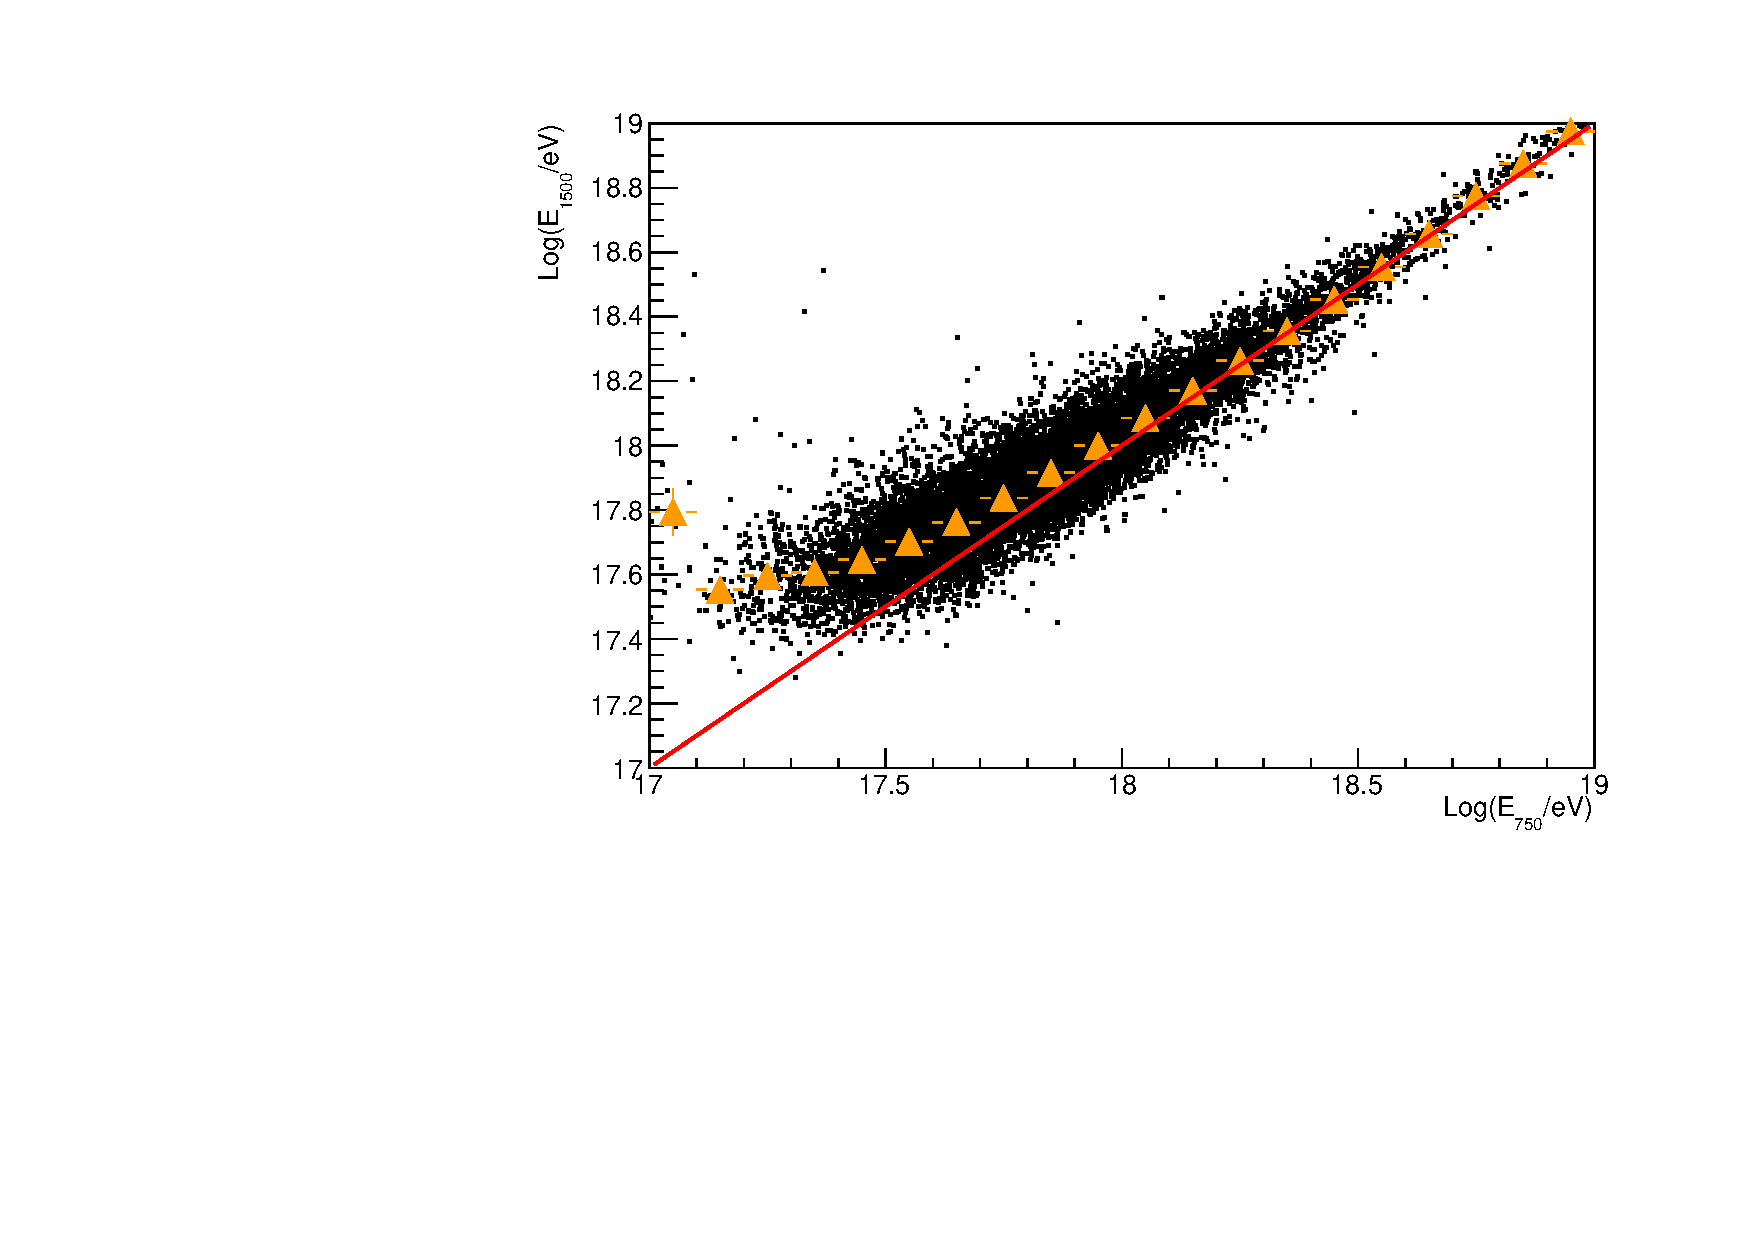
\includegraphics[width=0.7\textwidth]{plots/energy45.pdf}  
\caption{Energy measured by the SD1500 as a function of the energy measured by the SD750 toghether with it's average. In red it can be seen the identity function.
\label{fig:energy}}
\end{center}
\end{figure} 

\begin{figure}[h]
\begin{center}
 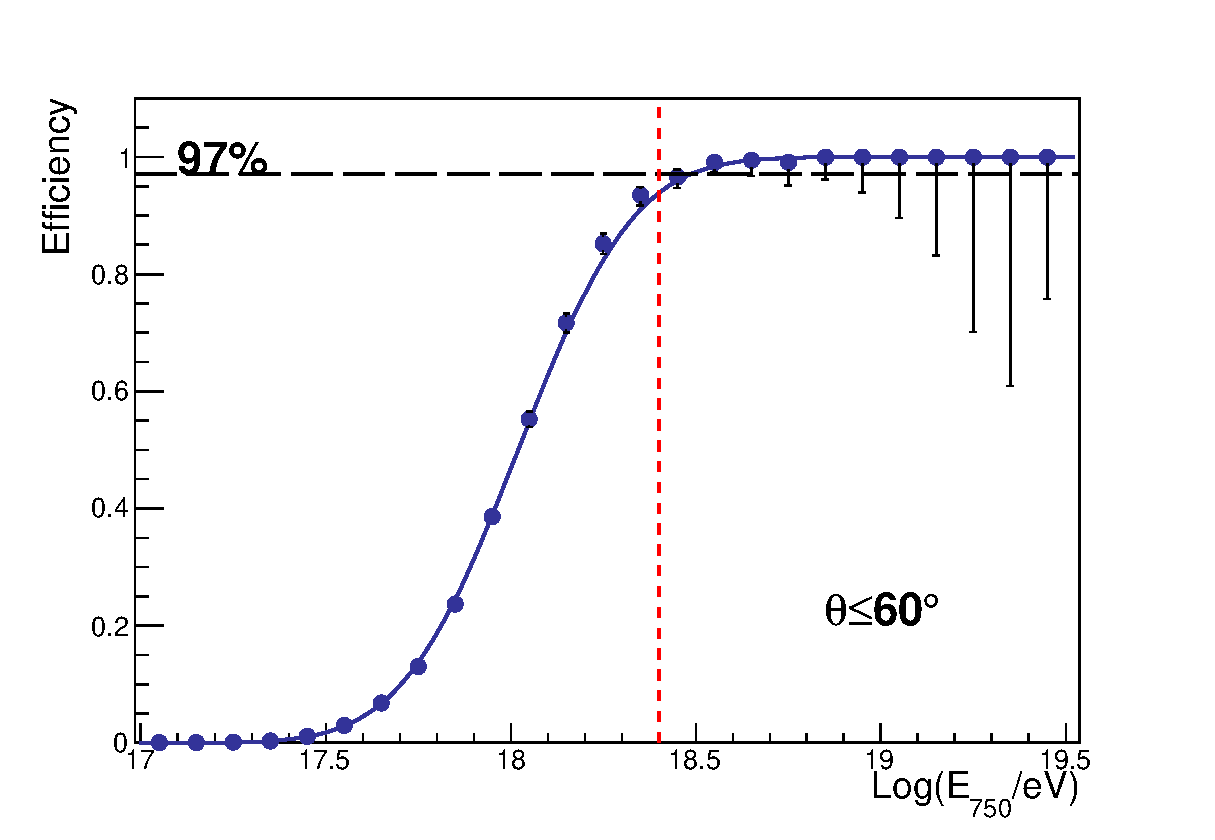
\includegraphics[width=0.7\textwidth]{plots/allZenith.eps}  
\caption{SD1500 efficiency measured with the SD750 event set. The $97\%$ efficiency threshold to report the spectrum is reached in the $10^{18.4}\eV$ bin.
\label{fig:allZenith}}
\end{center}
\end{figure} 

% \begin{figure}[h]
% \begin{center}
%  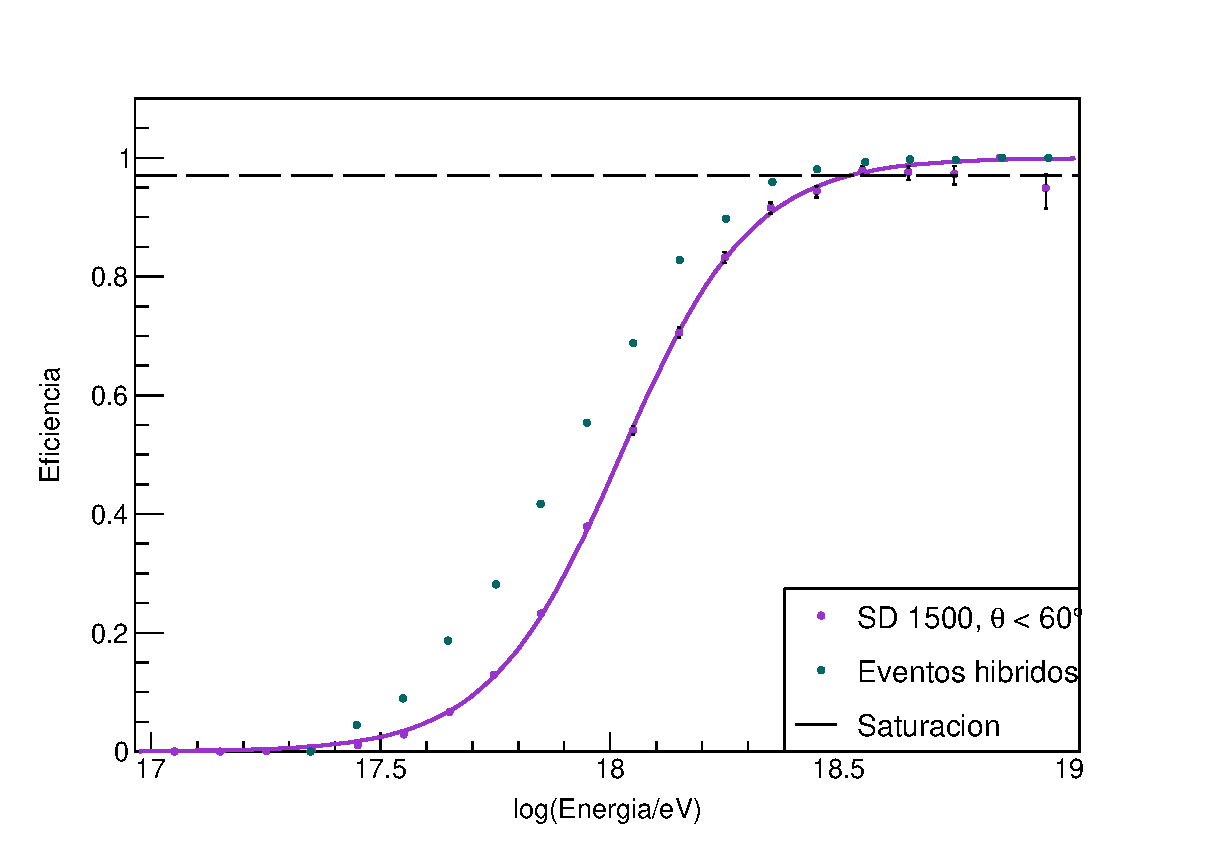
\includegraphics[width=0.7\textwidth]{plots/Hibridos.eps}  
% \caption{   
% \label{fig:hybrid}}
% \end{center}
% \end{figure} 


\section{Zenith angle dependence of the efficiency}
\label{sec:zenith}

\begin{figure}[]
\center
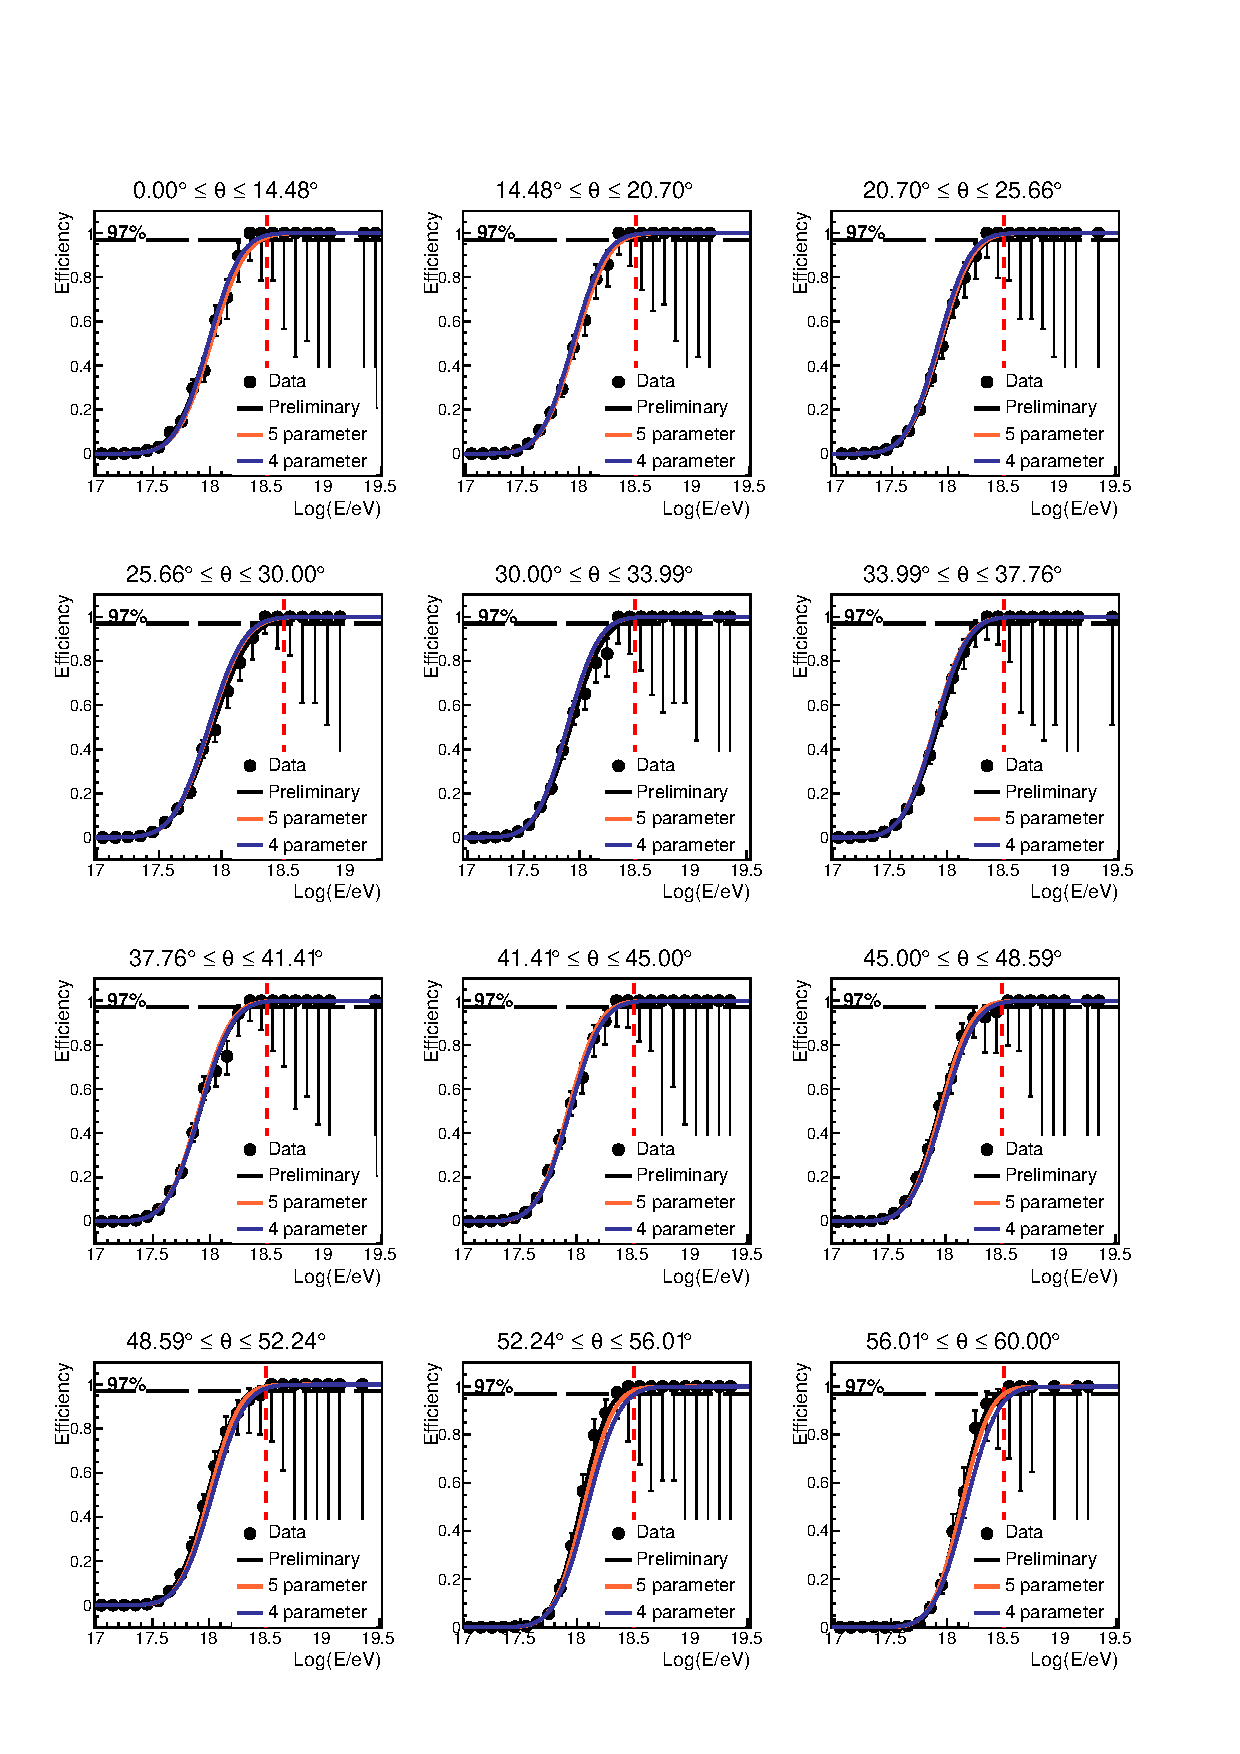
\includegraphics[width=0.99\textwidth]{plots/EfficiencyZenith.pdf}
\caption{SD1500 efficiency for zenith angle bins and the 4 and 5 parameter fittings proposed together with the preliminary fit.
\label{fig:zenith}}
\end{figure}



\begin{figure}[h]
\begin{center}
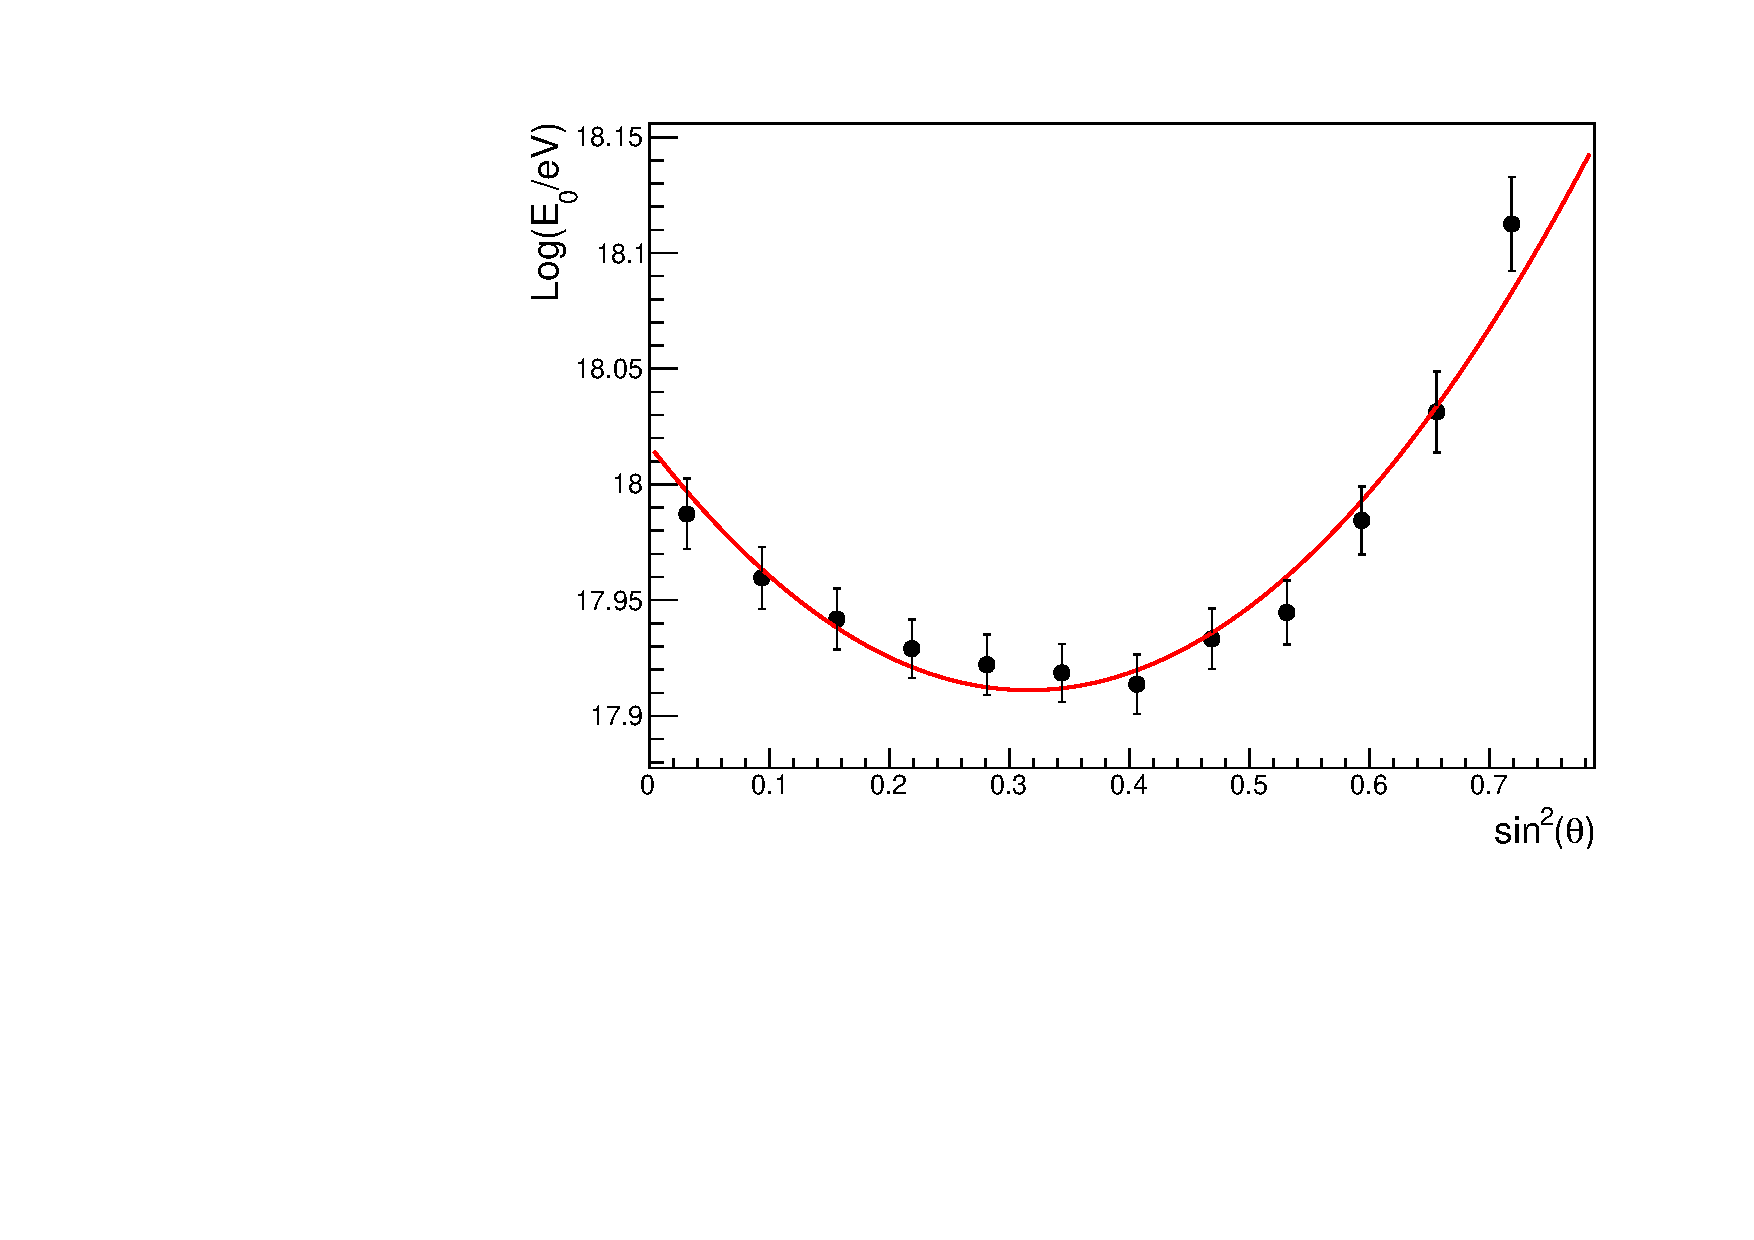
\includegraphics[width=0.49\textwidth]{plots/E0.pdf}
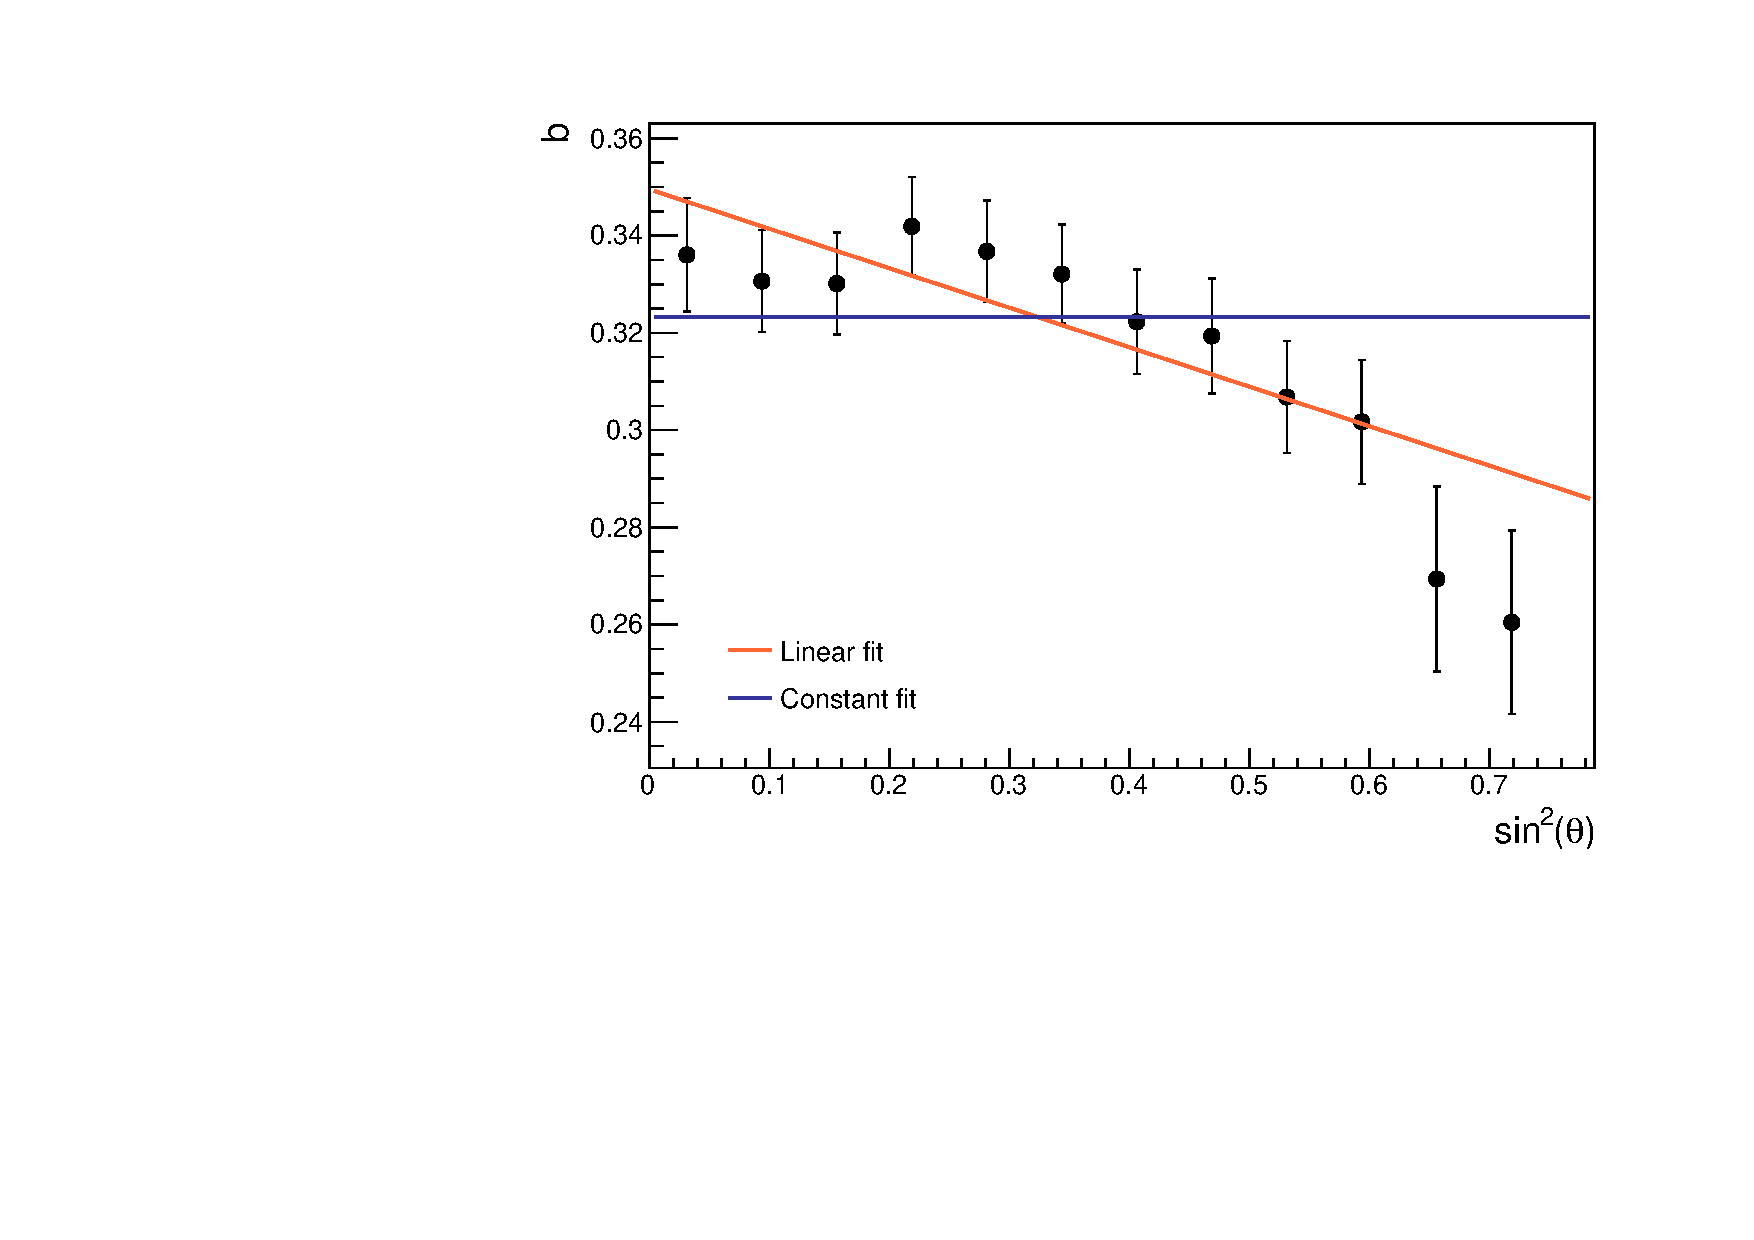
\includegraphics[width=0.49\textwidth]{plots/b.pdf}
\caption{Parameter deppendency with $\sin^2(\theta)$ for the prelminiary fit. $E_0$ shows a quadratic dependance and $b$ is modeled by a constant function and a linear function.
\label{fig:parameters}}
\end{center}
\end{figure} 



\begin{figure}[h]
\begin{center}
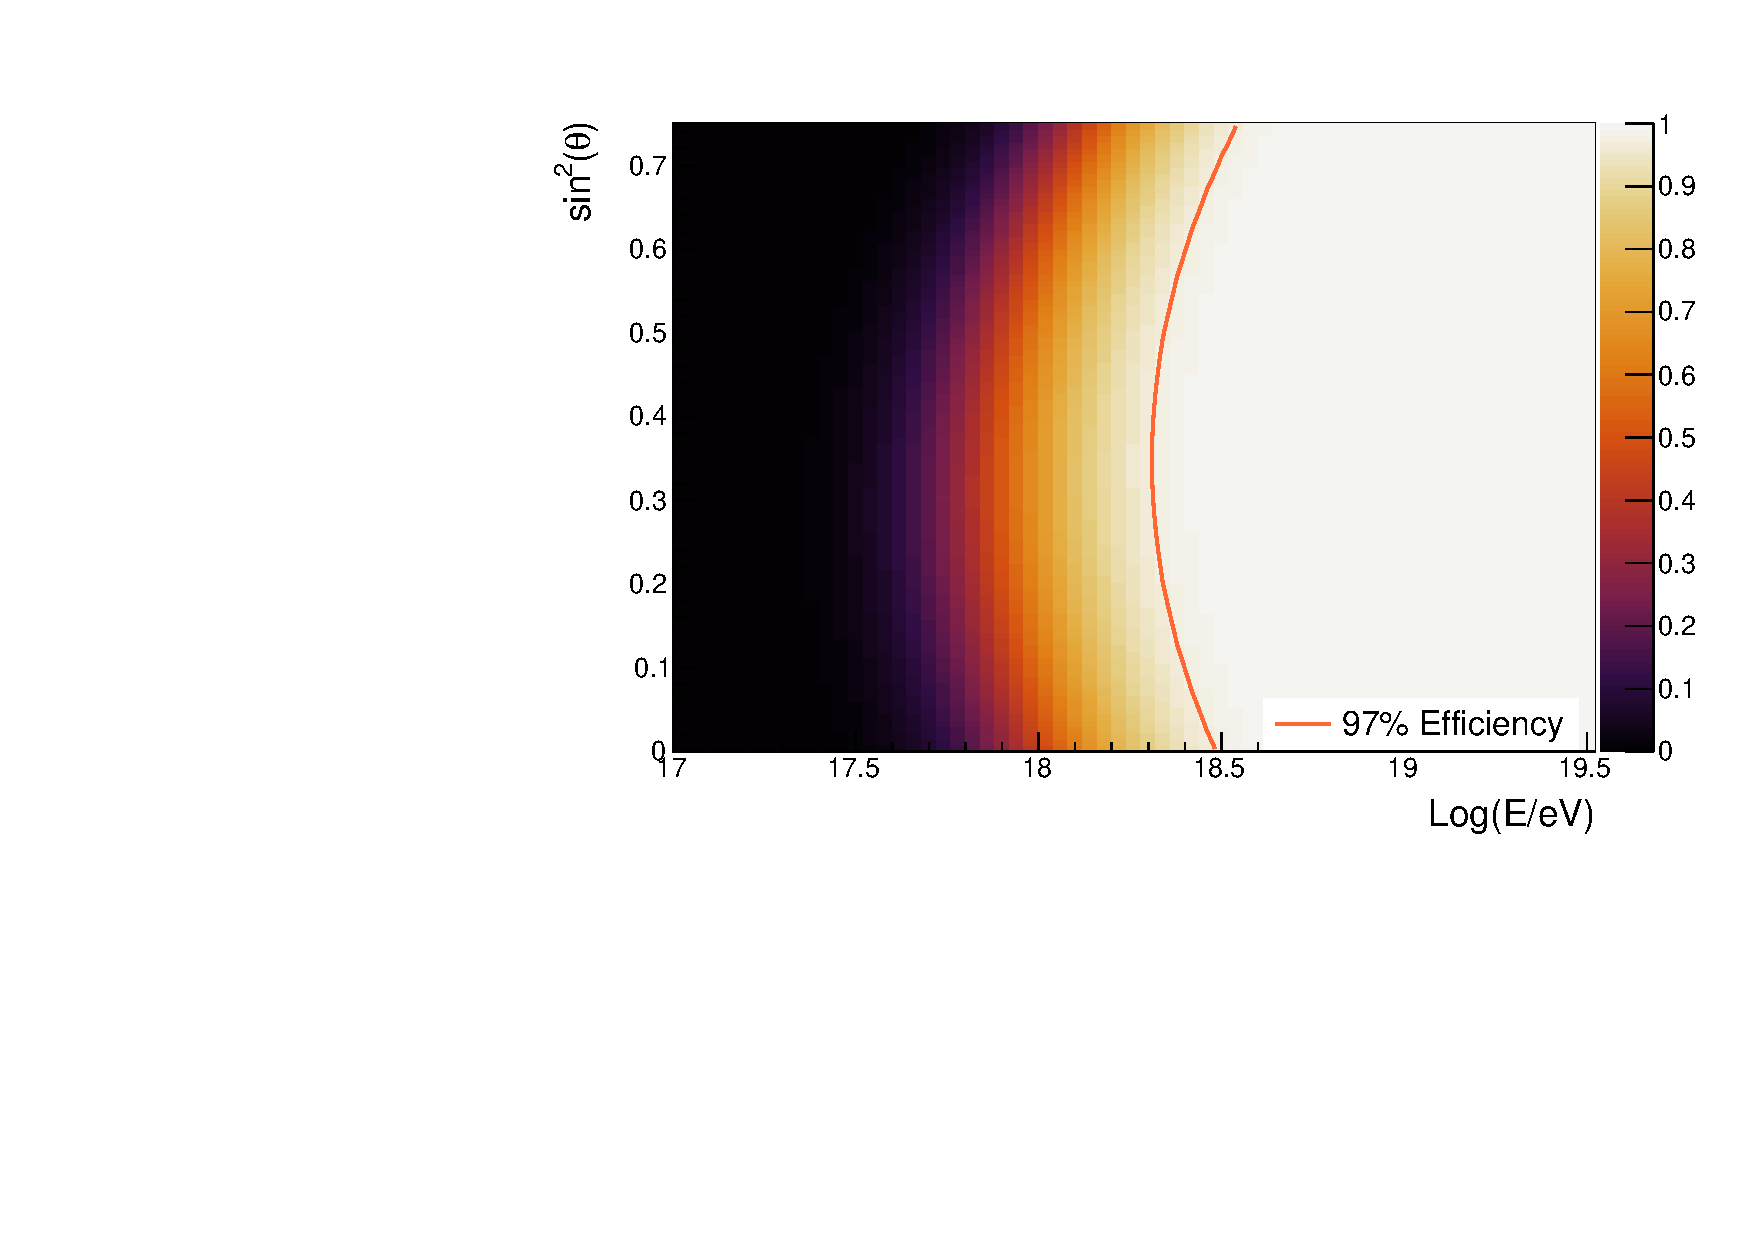
\includegraphics[width=0.7\textwidth]{plots/Surface.pdf}
\caption{Surface plot of the efficiency 5 parameter fit as a function of the energy and zenith angle toghether with the $97\%$ efficiency threshold for 4 and 5 parameter fit.
\label{fig:surface}}
\end{center}
\end{figure}  

\section{Efficiency of the 1500-metre array with the inclusion of the new triggers}
\label{sec:new}

\begin{figure}[h]
\begin{center}
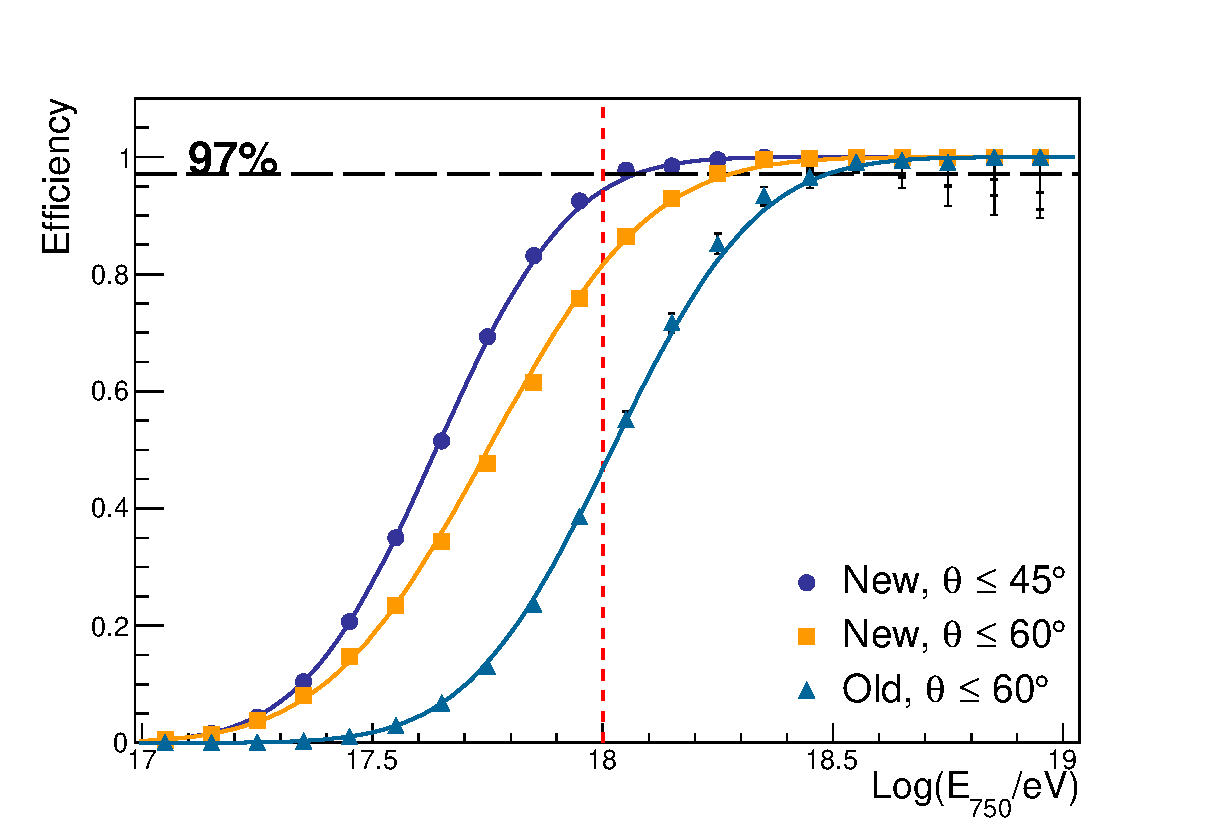
\includegraphics[width=0.7\textwidth]{plots/NewCut.eps}
\caption{SD1500 efficiency for events reconstructed including the new triggers for $\theta\leq60^\circ$ and the new zenith angle cut proposed $\theta\leq45^\circ$. The efficiency threshold is reached at $10^{18.2}\eV$ and $10^{18}\eV$ respectively.
\label{fig:NewCut}}
\end{center}
\end{figure}


\section{Efficiency correction of the SD-1500 Spectrum}
\label{sec:spectrum}

\begin{figure}[hb]
\begin{center}
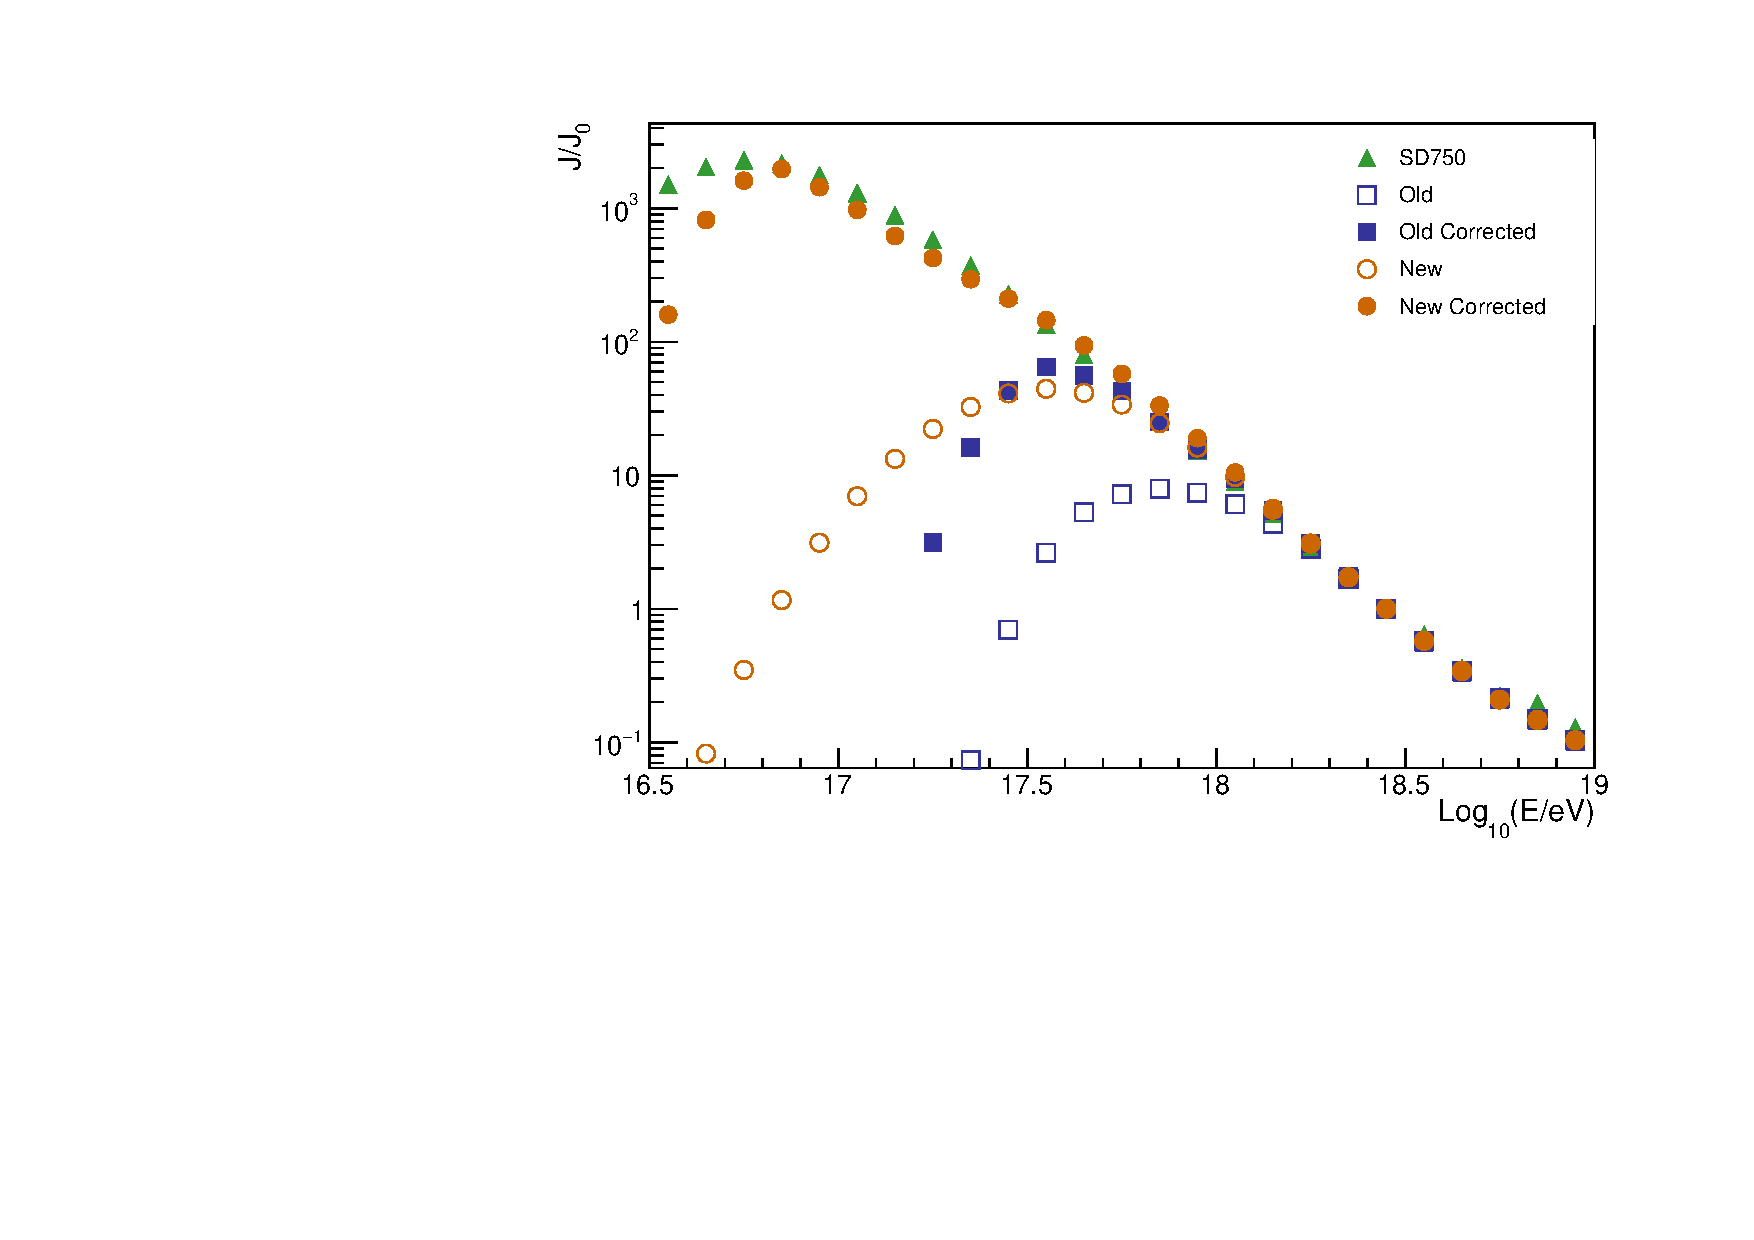
\includegraphics[width=0.7\textwidth]{plots/spectrum.pdf}
\caption{
\label{fig:flux}}
\end{center}
\end{figure}

\begin{figure}[h]
\begin{center}
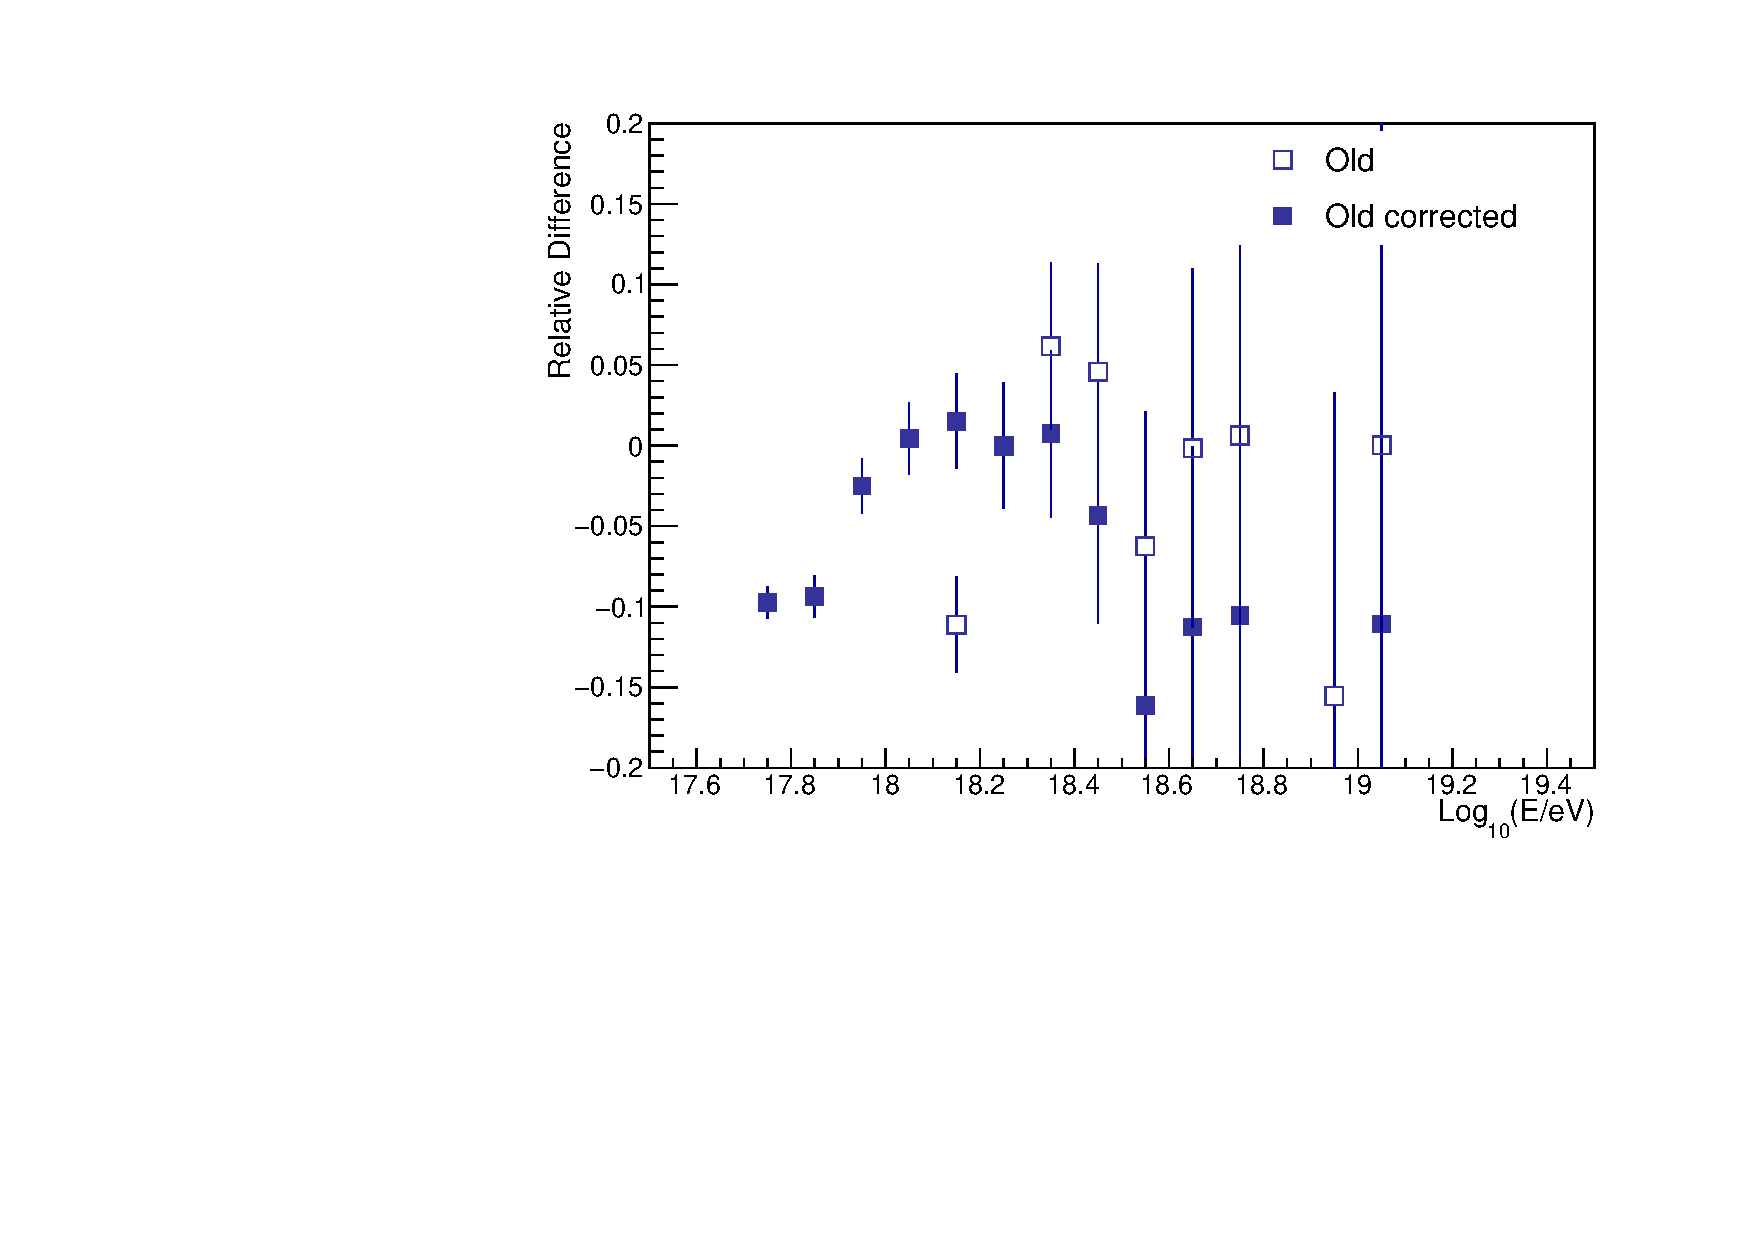
\includegraphics[width=0.7\textwidth]{plots/differenceOT.pdf}
\caption{
\label{fig:difference}}
\end{center}
\end{figure} 


\section*{Appendix: New Triggers}

\begin{figure}[h]
\begin{center}
 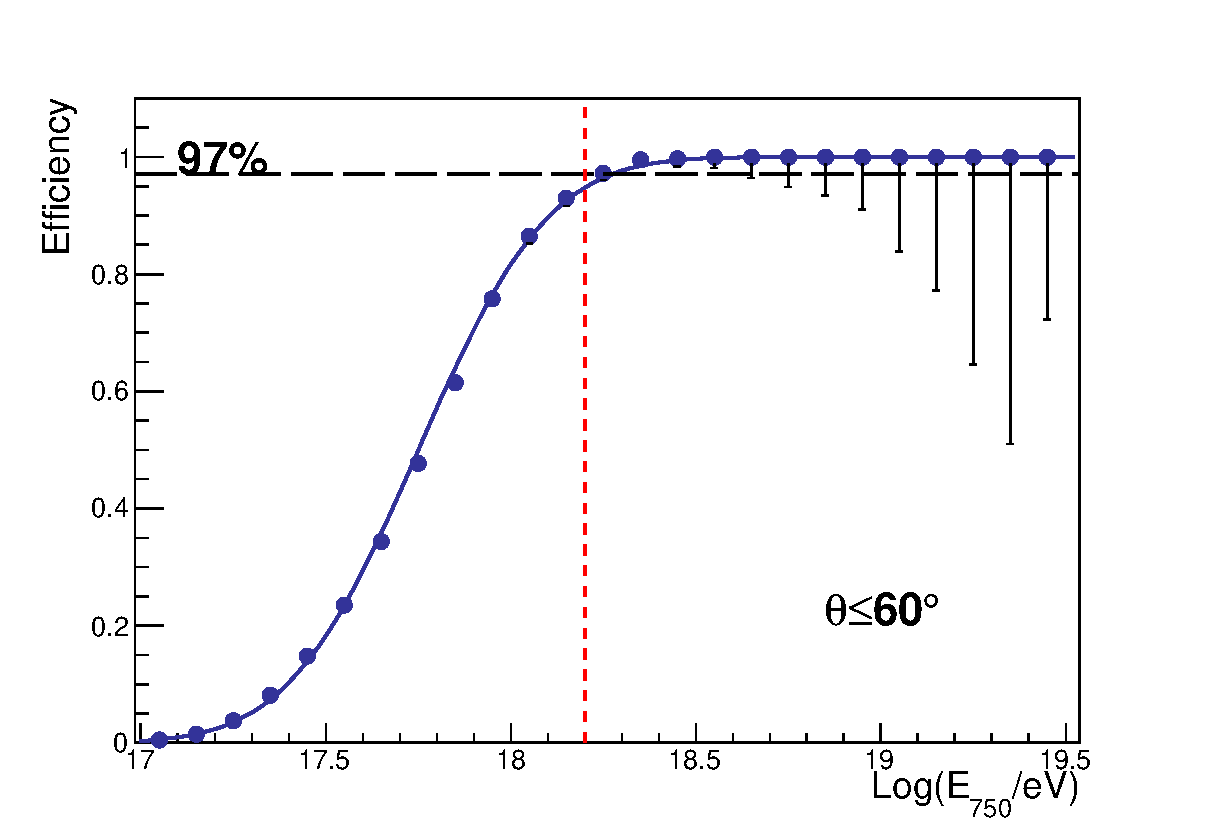
\includegraphics[width=0.7\textwidth]{plots/allZenithNew.eps}  
\caption{   
\label{fig:allZenithNew}}
\end{center}
\end{figure}

\begin{figure}[p]
\begin{center}
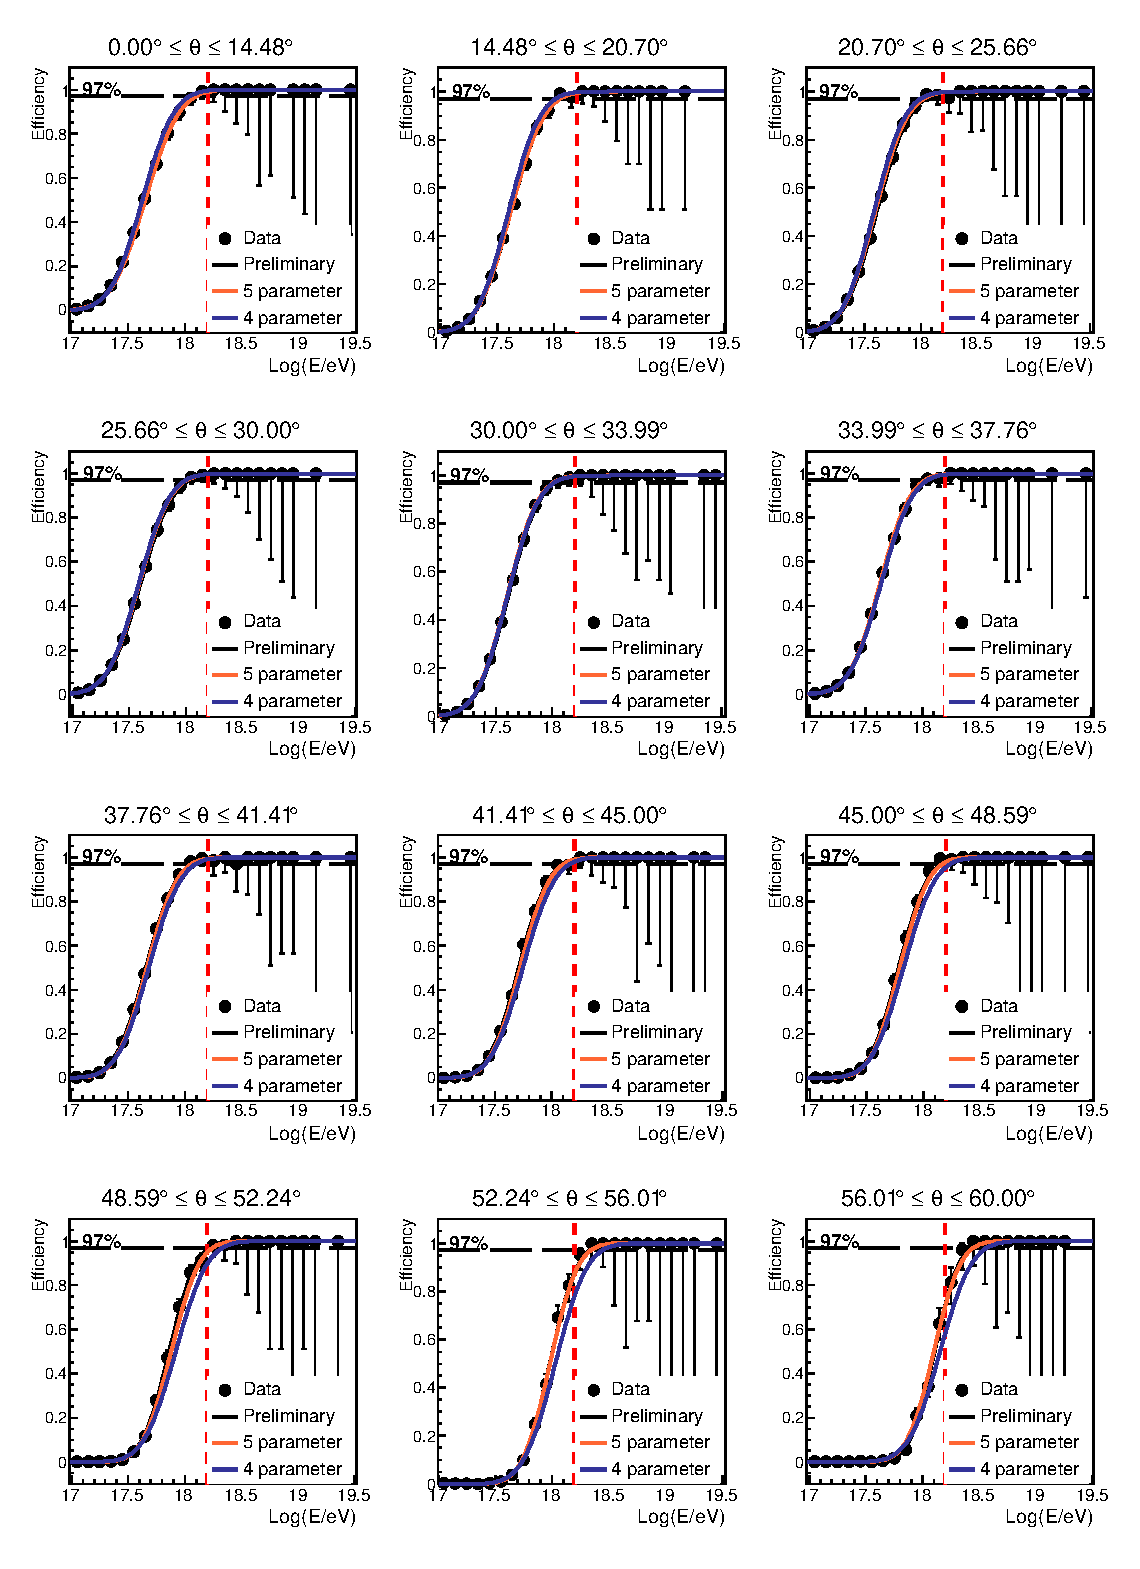
\includegraphics[width=\textwidth]{plots/EfficiencyZenithNew.eps}
\caption{
\label{fig:zenithNew}}
\end{center}
\end{figure}

\begin{figure}[h]
\begin{center}
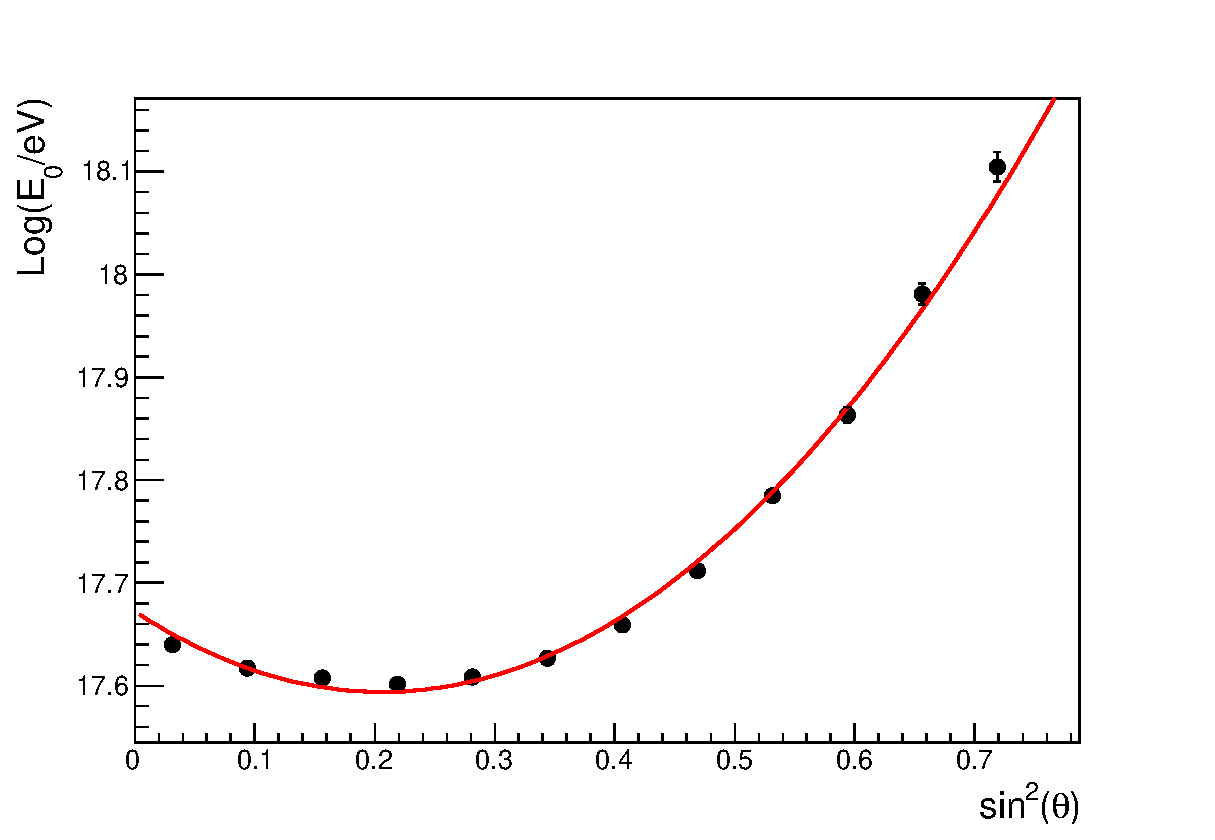
\includegraphics[width=0.49\textwidth]{plots/E0New.eps}
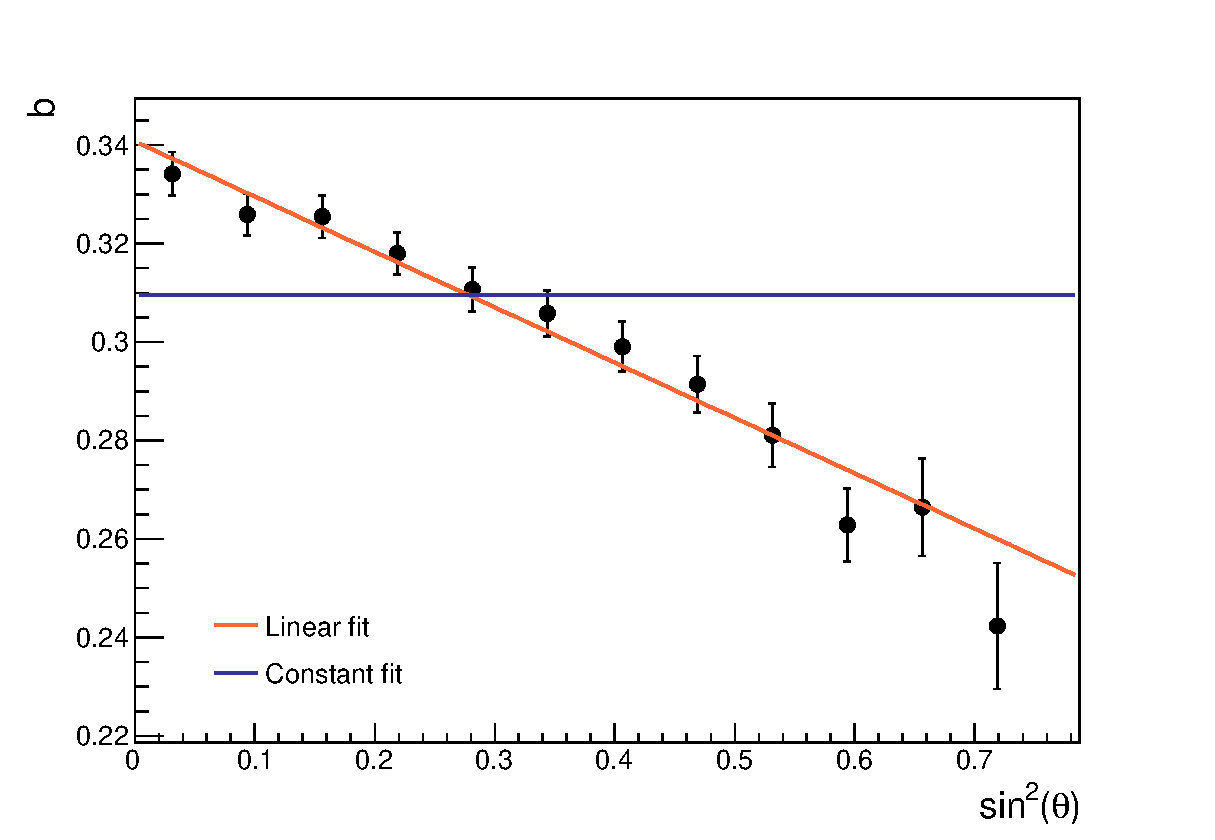
\includegraphics[width=0.49\textwidth]{plots/bNew.eps}
\caption{
\label{fig:parametersNew}}
\end{center}
\end{figure} 

\begin{figure}[h]
\begin{center}
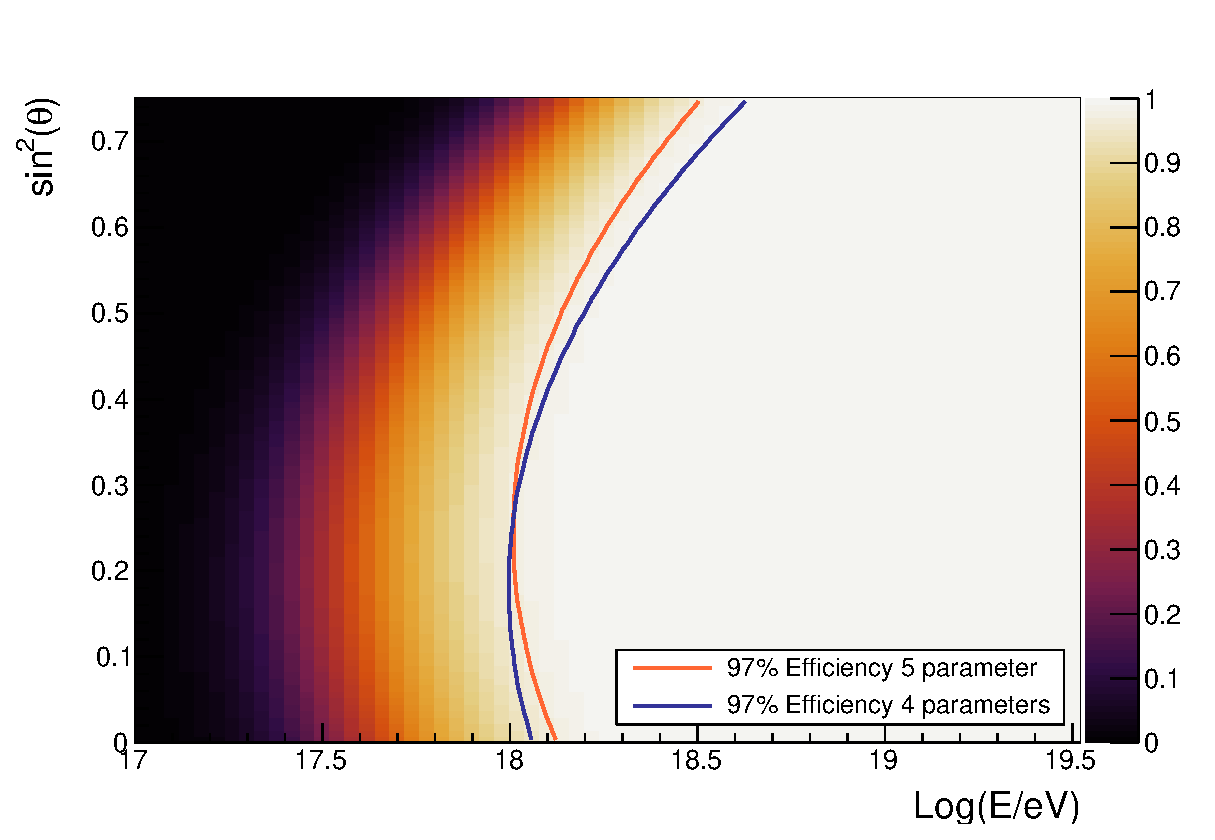
\includegraphics[width=0.7\textwidth]{plots/SurfaceNew.eps}
\caption{
\label{fig:surfaceNew}}
\end{center}
\end{figure}


\begin{thebibliography}{99}

\end{thebibliography} 

\end{document}
